\chapter{Morphological diversity in tenrecs compared to their closest relatives}
\label{chap:disparity}

%Changed this chapter to be based on the paper after comments from NC
\section{Introduction}
%SF: I haven't repeated the paper's introduction here because it's in the introduction of my thesis instead - do I need a separate introduction for this chapter since it's a continuation of the main introduction and methods chapter?

	It is important to study patterns of morphological diversity to gain a greater insight into species' evolutionary histories and ecological interactions (chapter \ref{chap:introduction}). 
	
	In this chapter, I present the first quantitative investigation of morphological diversity in tenrecs. I use geometric morphometric techniques \citep{Rohlf1993} to compare cranial morphological diversity in tenrecs to their closest relatives, the golden moles. Tenrecs inhabit a wider variety of ecological niches thank golden moles \citep{Soarimalala2011, Bronner1995} so I expected tenrecs to be more morphologically diverse. However, tenrecs only had higher morphological diversity than golden moles for some but not all views of skull shape. Further analyses (see section \ref{sect:results}) revealed that the morphological similarities within the \textit{Microgale} tenrec Genus appears to reduce the overall morphological diversity of the Family as a whole.
	%Needs one more sentence to finish off the introduction

%------------------------------------------------------
\section{Methods}

	I have already described how I photographed crania and summarised their morphologies using landmark morphometrics (chapter \ref{chap:methods}). In total, I photographed 99 different species from seven different mammal Families (table \ref{tab:species.measured}). However, here I am I only comparing the morphological diversity of tenrecs to their closest relatives, the golden moles. Some skulls were partly damaged and therefore I could not compare them in all of the separate views (dorsal, ventral and lateral) so the exact number of skulls that I used varies slightly for each measure. I used photographs of 182 skulls in dorsal view (148 tenrecs and 34 golden moles), 173 skulls in ventral view (141 tenrecs and 32 golden moles), 171 skulls in lateral view (140 tenrecs and 31 golden moles) and 181 mandibles in lateral view (147 tenrecs and 34 golden moles). These samples represent 31 species of tenrec (out of the total 34 in the Family \citep{Olson2013}) and 12 species of golden moles (out of a total of 21 species in the Family, \citep{Asher2010}).

	%Methods chapter describes everything up to the PC analysis: but maybe I should repeat some of that here and refer to the diagram
	
	%Put in the flow chart and revised methods text
	
%----------------------------------------------------

\section{Results}
\label{sect:results}
	%Edited these from the paper comments
	%Change to using all four PCA plots

	Figure \ref{fig:FourPCA} depicts the morphospaces defined by the first two principal component (PC) axes from my principal components analyses (PCAs) of skull and mandible morphologies. The PCAs are based on the average Procrustes-superimposed shape coordinates for skulls in three views (dorsal, ventral and lateral) and mandibles in lateral view.

%-----------------------------
%New PCA figure: all four PCAs together, pictures as legend, bigger axis labels
%I haven't put in the warp diagrams because they made it too crowded. I could add warps if I put in each PCA as a separate plot
	
%PCA figure: Just sklat as an example
	%From the twofamily_disparity_PCAplots script
	\begin{figure}[!htbp]
	\centering
	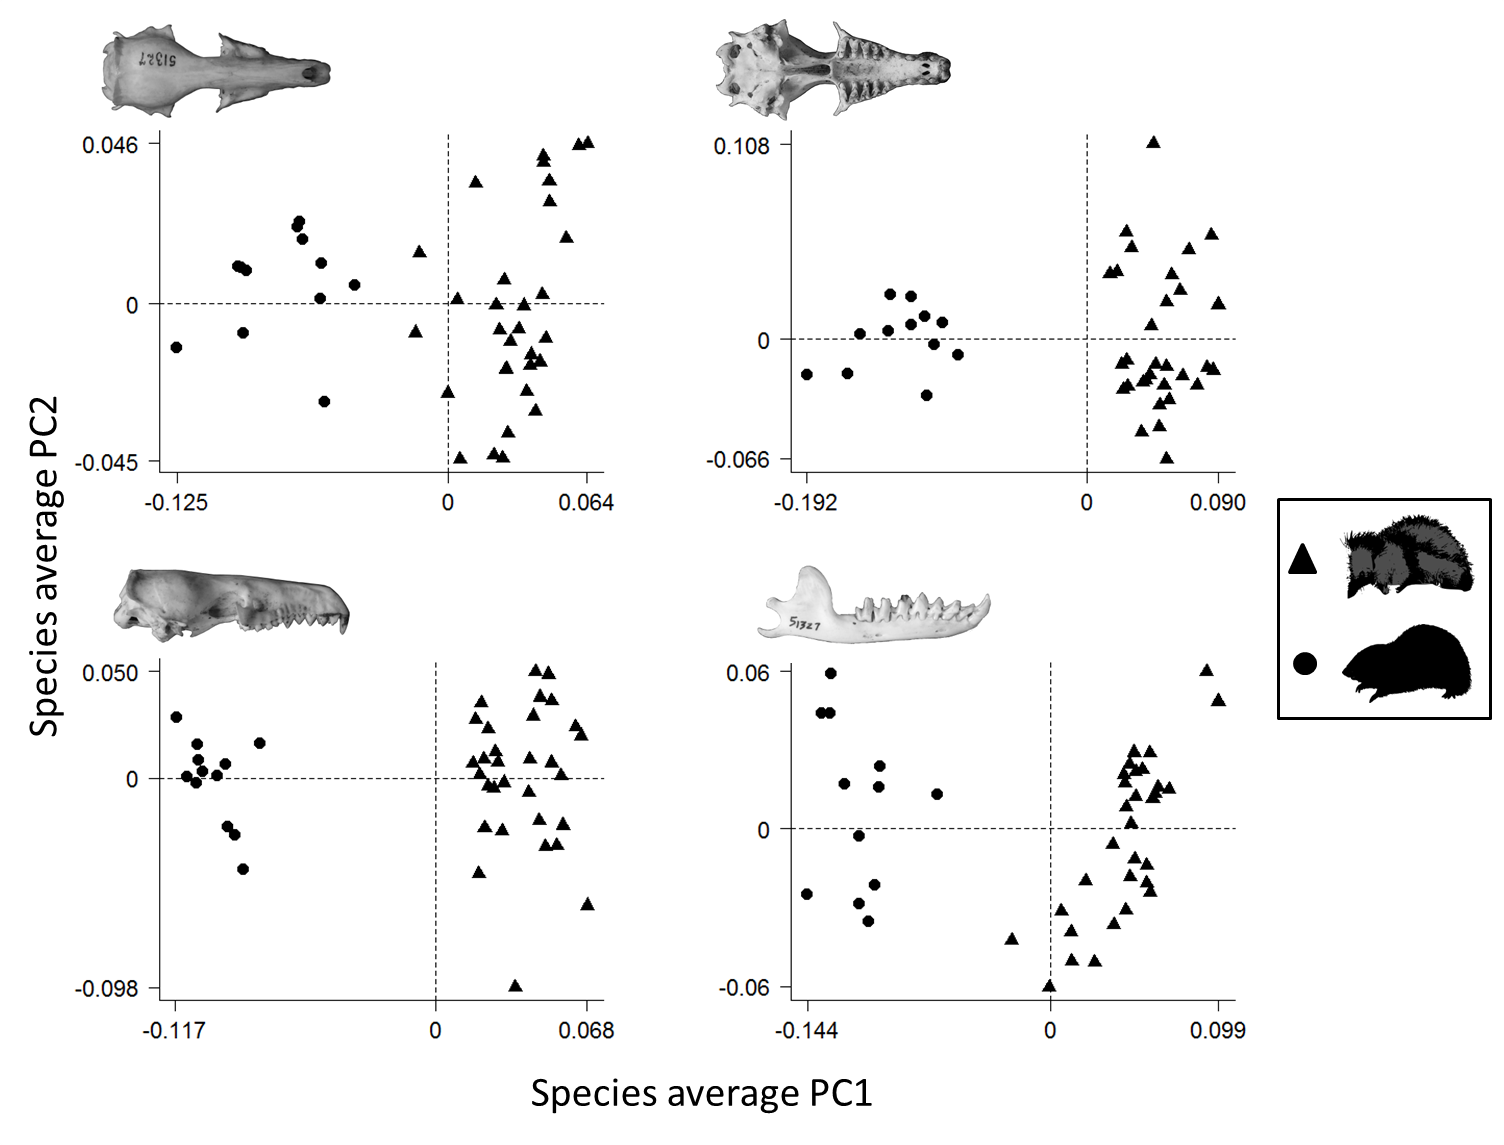
\includegraphics[width=1\linewidth]{Disparity/writing/figures/FourPCA_shapes.png}
	\caption[Morphospace (principal components) plot of morphological diversity in lateral views of tenrec and golden mole skulls.]
		{Principal components plots of the morphospaces occupied by tenrecs (triangles, n=31 species) and golden moles (circles, n=12) for the skulls (dorsal, ventral and lateral views) and mandibles (lateral view). Each point represents the average skull shape of an individual species. Axes are principal component 1 and principal component 2 of the average scores from Principal Components Analyses of mean Procrustes shape coordinates for each species.}
	\label{fig:FourPCA}
	\end{figure}
%----------------------------------------------

	To compare morphological diversity in the two families, I used the PC axes which accounted for 95\% of the cumulative variation in each of the skull analyses: dorsal (n=6 axes), ventral (n=7 axes) and lateral (n=7 axes) and the mandibles (n=11 axes).
	
	First, I compared the position of each Family within the morphospace plots. Tenrecs and golden moles occupy significantly different positions in the dorsal (npMANOVA, F \textsubscript{1,42} = 68.13, R$^2$ =0.62, p=0.001 ), ventral (npMANOVA, F \textsubscript{1,42} = 103.33, R$^2$ =0.72 , p=0.001 ) and lateral (npMANOVA, F \textsubscript{1,42} = 76.7, R$^2$ =0.652, p=0.001 ) skull morphospaces as well as in the mandible morphospace (npMANOVA, F \textsubscript{1,42} = 60.38, R$^2$ =0.59, p=0.001),  indicating that the Families have very different, non-overlapping cranial and mandible morphologies. 
	
	%Numbers are from the npMANOVA based on PC axes within my diversity_twofamily_cent_dist script

	Secondly, I compared the morphological diversity within each Family. Based on my measures of mean Euclidean distance to the Family's centroid, tenrec skulls are more morphologically diverse than golden mole skulls when they are measured in lateral view but not in dorsal or ventral view (table \ref{tab:diversity}). In contrast, when I analysed morphological diversity of skulls within the sub-sample of 17 tenrecs (including just five \textit{Microgale} species) compared to the 12 golden mole species, I found that tenrec skulls were significantly more morphologically diverse than golden moles in all analyses (table \ref{tab:diversity}).
	
%----------------------------------------
%Results table: I changed the format of the first one to make it fit better
	\begin{table}[!htbp]			
		\caption[Comparison of morphological diversity in tenrecs and golden moles.]
		{Morphological diversity in tenrecs compared to golden moles. I repeated each analysis with the full data (31 tenrec species) and then with 17 tenrec species (including just five species from the \textit{Microgale} genus). In each case, I compared the morphological diversity in tenrecs to the diversity within 12 species of golden moles. Significant differences between the two Families (p $<$ 0.05) are highlighted in bold.}
		%Diversity based on centroid distances results summary
%All tenrecs and golden moles
%Morphological diversity based on comparing the mean Euclidean distances to each family's centroid
%NB: degrees of freedom are different in each analysis because I'm using a Welch two sample t test: df comes from a distribution of values based on the error within each sample so the final numbers will be different for each data set

%Re-ordered the table so that everything would fit in better


\resizebox{\columnwidth}{!}{
%Scales down the table to fit within the column width
	% If this is too small then I'll probably need to break the table into two
\begin{tabular}{c l c c c c}		
\hline
N& Analysis & \multicolumn{2}{c}{Morphological diversity} & t\textsubscript{df} & p value\\
%-----------------------------------------------
\hline
%------------------------
 &  & Tenrecs  & Golden moles &  &  \\
%--------------------------------
\cline{3-4} % Puts a line just through some columns
%---------------------------------
 & & (mean $\pm$ s.e) & (mean $\pm$ s.e) & &\\
\hline
%\multicolumn{1}{l}
%---------------------------
 31 & Skulls dorsal & \multicolumn{1}{l}{0.036 $\pm$ 0.0029} & 0.029 $\pm$ 0.0032 & -1.63\textsubscript{29.88}& 0.11 \\
%--------------------------------------
 & Skulls ventral & \multicolumn{1}{l}{0.048 $\pm$ 0.0034} & 0.044 $\pm$ 0.0041 & -0.68\textsubscript{26.99} & 0.51\\
%-----------------------------------------
 & Skulls lateral & 0.044 $\pm$ 0.0041 & 0.032 $\pm$ 0.0037 & -2.16\textsubscript{35.03} & \textbf{0.04}\\
%----------------------------------------
 & Mandibles & 0.049 $\pm$ 0.0044 & 0.067 $\pm$ 0.0054 & 2.62\textsubscript{25.85} & \textbf{0.01}\\
%--------------------------
\hline
%-----------------------------------------
17 & Skulls dorsal & 0.044 $\pm$ 0.0025 & \multicolumn{1}{l}{0.029 $\pm$ 0.0032} & -3.62\textsubscript{22.75} & \textbf{<0.01}\\
%---------------------------------
 & Skulls ventral & \multicolumn{1}{l}{0.054 $\pm$ 0.0039} & \multicolumn{1}{l}{0.042 $\pm$ 0.0041} & -2.23\textsubscript{25.46} & \textbf{0.04}\\
%-------------------------------------
 & Skulls lateral &  \multicolumn{1}{l}{0.054 $\pm$ 0.0053} & 0.031 $\pm$ 0.0037 & -3.47\textsubscript{26.31} & \textbf{<0.01} \\
%--------------------
 & Mandibles & 0.055 $\pm$ 0.0049 & \multicolumn{1}{l}{0.062 $\pm$ 0.0050} & 1.00\textsubscript{25.88} & 0.33 \\
%--------------------

\hline
\end{tabular}
} 
		\label{tab:diversity}  
	\end{table}
%------------------------------------	
	The results of my analyses of the mandibles were different to those for the skulls. In the full analysis (31 species of tenrec compared to 12 species of golden mole), I found that golden moles have significantly more diverse mandible shapes than tenrecs but this difference was not significant when I used just 17 tenrec species (table \ref{tab:diversity})
	

	The pairwise permutation tests for each analysis confirmed that differences in morphological diversity were not artefacts of differences in sample size table \ref{tab:permutations}.
	

%Added the permutation results
\begin{table}[!htbp]			
	\caption[Results of the permutation tests]{Results of the permutation analyses which compared the observed differences in morphological diversity to a null distribution of expected results. I repeated the permutation comparisons for both the full (31 species of tenrec compared to 12 species of golden mole) and reduced (17 species of tenrec compared to 12 golden moles) data sets. In each case, the observed differences in morphological diversity were significantly different to the expected differences under a null hypothesis (significant p values). Therefore, the differences in morphological diversity between the two Families were not just artefacts of differences in sample size.}
	%Combined table of permutation results

\resizebox{\columnwidth}{!}{
\begin{tabular}[t]{l l c c c c c c c}		
\hline
%------------------------------------------
N & Analysis & \multicolumn{5}{c}{Morphological diversity} & p value\\
%-------------------
\hline
%-------------------------------------------
 &  & \multicolumn{3}{c}{Measured values}& \multicolumn{2}{c}{Permuted values} &  \\
%---------------
\cline{3-7}
%-----------------
& & Tenrecs & Golden moles & Difference & Min. & Max. & \\
\hline
%--------------------------------------------------------
31 & Dorsal & 0.036 & 0.029 & 0.007 & -0.011 & 0.0098 &  0.013 \\
%--------------------------------------------------------
& Ventral &  0.048 & 0.044 & 0.0036 & -0.014 & 0.013 &  0.023\\
%--------------------------------------------------------
& Lateral & 0.044 & 0.032 & 0.012 & -0.012 & 0.011 & <0.001 \\
%--------------------------------------------------------
& Mandibles & 0.049 & 0.067 & 0.018 & -0.008 & 0.009  & <0.001 \\
%-----------------------------
\hline
%--------------------------------------------------------
17 & Dorsal & 0.044 & 0.029 & 0.015 & -0.011 & 0.014 &  <0.001 \\
%--------------------------------------------------------
& Ventral &  0.054 & 0.042 & 0.013 & -0.017 & 0.019 &  0.023 \\
%--------------------------------------------------------
& Lateral & 0.054 & 0.0313 & 0.022 & -0.018 & 0.0186 & <0.001 \\
%--------------------------------------------------------
& Mandibles & 0.055 & 0.0623 & 0.007 & -0.012 & 0.011 & 0.038\\
%-----------------------------
\hline
\end{tabular}
} 
	\label{tab:permutations}  
\end{table}
	
%----------------------------------------------------

\section{Discussion}

%I wasn't sure how much discussion to put in here and how much to leave for the separate chapter.
%I could just do a brief summary here and leave the rest for the separate chapter
%Or I could deal with most of the technical and interpretation issues here and then the last chapter would just be a short summary and then more information on future directions/ expansion of the project



